\documentclass{fhnwreport}
\usepackage[ngerman]{babel}
\usepackage[T1]{fontenc}
\usepackage[utf8]{inputenc}
\usepackage{tikz}
\usetikzlibrary{arrows}
\usepackage{amsmath}
\usepackage{lmodern}
\usepackage[final]{pdfpages}
\usepackage{graphicx}
\usepackage{textcomp}
\usepackage{multirow}
\usepackage{todonotes}
\usepackage{pdfpages}
\bibliographystyle{IEEEtran}
\usepackage{cite}
\usepackage[nottoc,notlof,notlot,numbib]{tocbibind}
%\usepackage[nottoc, numbib]{tocbibind}

\title{%
  \textsc{Laborfähiger Photovoltaiksimulator}\\
  \textsc{Pflichtenheft}}
\author{%
  \textsc{Projekt 3 - Team 3}\\
  \textsc{Simon Sturm, Yanick Frei,
Claudius Jörg}}
\date{%
  \textsc{Windisch, 08.10.2015}}

\begin{document}
\begin{center}
\Large Laborfähiger Photovoltaiksimulator\\
Pflichtenheft\\
\large Projekt 3 - Team 3\\
Simon Sturm, Yanick Frei, Claudius Jörg\\
Windisch, 08.10.2015
\end{center}


\textbf{Lösungskonzept}
\begin{itemize}
	\item Das Gerät hat eine interne Versorgungsspannung von 24V.
	\item Es wird ein variabler Schaltregler zur Spannungseinstellung benutzt.
	\item Strom und Spannung werden mittels MC geregelt:\\
	Falls Strom und Spannungswerte nicht übereinstimmen passt der	Mikrocontroller die Spannung an, bis diese mit dem gewünschten Strom übereinstimmt (Wertetabelle).
		\item Ein Printlayout für die Serienproduktion wird erstellt.
		Falls genügend Zeit vorhanden ist, wird dieses auch bestückt und getestet.
		\item Die Bedienung des Gerätes erfolgt mit zwei Tastern (+/-), mit denen die Bestrahlungsstärke eingestellt werden kann (20-100 Prozent). Die eventuelle Verschmutzung oder Teildefekte werden ebenfalls mit Tastern aktiviert.
		\item Das Gerät kann mittels Hauptschalter ein- und ausgeschaltet werden.
		\item Spannungs- und Stromwerte sowie die momentane Bestrahlungsstärke werden auf einem 4-Zeiligen Display ausgegeben.
		\item Die Steuerung wird mittels Mikrocontroller erledigt.%\\
		%Dieser liest die beiden Taster ein und regelt dementsprechend den Ausgang des Spannungsreglers. Weiterhin liest er die Ausgangsspannung des Messgerätes über den internen AD Wandler ein und nimmt entsprechende Anpassungen am Regler vor.
\end{itemize}

\textbf{Hardwarekonzept}\\
\begin{center}
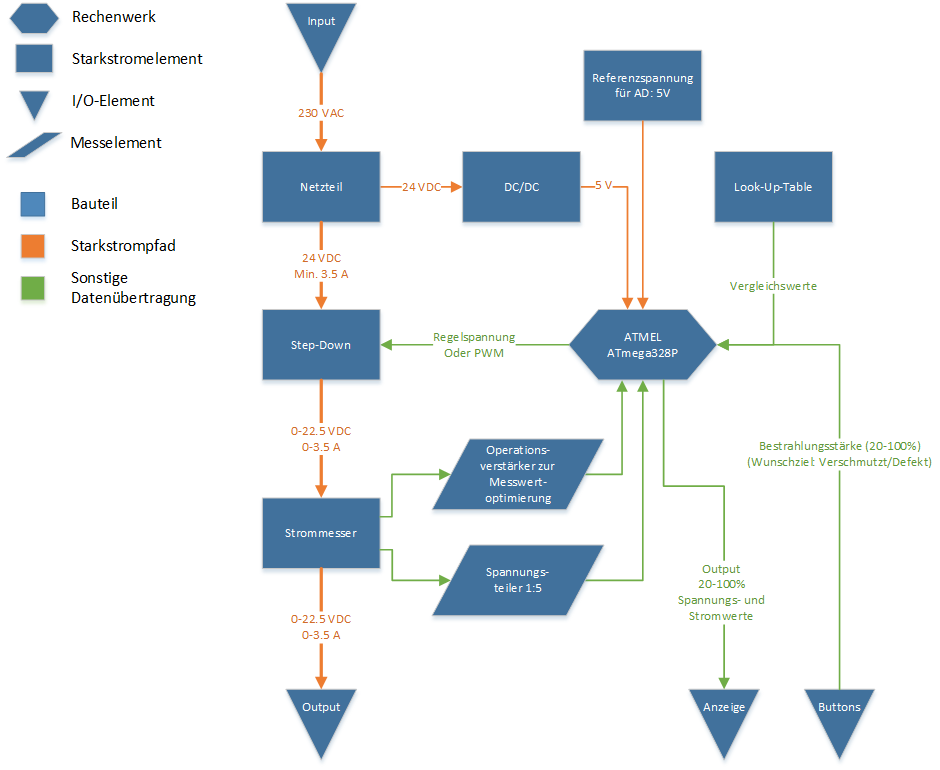
\includegraphics[scale=0.7]{Hardwarekonzept_V3}
\end{center}

\newpage
\textbf{Softwarekonzept}
\begin{itemize}
\item Beim Programmstart:
	\begin{itemize}
	\item Look-Up-Table mit Strom- und Spannungswerten laden (siehe unten).
	\item Display initialisieren
	\item Taster initialisieren
	\item Analoge Eingänge initialisieren
	\item Die Startspannung wird auf 5 Volt festgelegt.
	\end{itemize}

\item Andauernd wiederholen:
	\begin{itemize}
	\item Strom messen
	\item Spannung messen
	\item Displayanzeige aktualisieren
	\item Strom und Spannung in Look-Up-Table nachschlagen
	\item Falls Strom zu klein: Spannung erhöhen
	\item Falls Strom zu gross: Spannung verringern
	\item Kurzes Delay
	\end{itemize}
	
\item Beim Tasterdruck:
	\begin{itemize}
	\item Werte der Look-Up-Table entsprechend der Formel bearbeiten.
	\end{itemize}
	
\item Look-Up-Table:\\
In der Look-Up-Table sind für die entsprechenden Prozentwerte die zu den Stromwerten zugehörigen Spannungswerte hinterlegt.
\end{itemize}

\textbf{Testkkonzept}
\begin{itemize}
	\item Die einzelnen Schaltungsteile werden mittels LT Spice simuliert.
	\item Ein funktionsfähiger Prototyp wird mittels Lochrasterplatine erstellt.
	\item Die vorgängig notierten, zu erwarteten, Testwerte werden mit den Messergebnissen abgeglichen:
		\begin{itemize}
		\item Strom durch Stromwandler und entsprechende Ausgangsspannung am Stromwandler (185mV/A)
		\item Wert an OP Ausgang der Strommessung: 1.25V/Ampere
		\item Spannung an Spannungsteiler (0.2V/V)
		\item Stimmen der PWM-Ausgang des MCs und der Ausgang des Schaltreglers überein	(selber Duty-Cycle)
		\end{itemize}
	\item Alle Änderungen werden protokolliert, um den Lösungsweg nachvollziehbar gestalten zu können.
\end{itemize}

%\newpage
%\bibliography{literaturverzeichnis}
%\listoffigures
%\listoftables

\end{document}

